\documentclass[11pt,a4paper]{article}

\usepackage[utf8]{inputenc}
\usepackage[T1]{fontenc}
\usepackage[spanish]{babel}
\usepackage{geometry}
\usepackage{array}
\usepackage{longtable}
\usepackage{booktabs}
\usepackage{tabularx}
\usepackage{hyperref}
\usepackage{enumitem}
\usepackage{graphicx}
\usepackage{float}

\geometry{top=2.5cm,bottom=2.5cm,left=2.5cm,right=2.5cm}
\hypersetup{
	colorlinks=true,
	linkcolor=blue,
	urlcolor=blue,
	pdftitle={Elección del dataset},
	pdfauthor={Grupo de trabajo}
}

\renewcommand{\arraystretch}{1.15}
\setlength{\parindent}{0pt}
\setlength{\parskip}{0.65em}
\setlength{\emergencystretch}{2em}

\title{\textbf{Elección y Descripción del Conjunto de Datos, Grupo 1}}
\author{Matías López, Isidro Silicaro Pera, Taciano Pacchialat}
\date{}

\begin{document}

\maketitle

\section{Introducción al dominio: ¿Qué es la UFC?}

La \textbf{UFC} (\textit{Ultimate Fighting Championship}) es la organización de artes marciales mixtas (MMA, por sus siglas en inglés) más grande e importante del mundo. Las MMA son un deporte de combate que permite a los atletas utilizar técnicas de múltiples disciplinas marciales: golpeo de pie (como el boxeo o el kickboxing), lucha en pie (como el judo o la lucha olímpica) y combate en el suelo (como el jiu-jitsu brasileño o el wrestling).

\subsection*{Estructura de una pelea}

Cada enfrentamiento tiene lugar en un área de combate octagonal denominada \textbf{octágono}, con dos competidores ubicados en los llamados \textbf{rincón rojo} y \textbf{rincón azul}. Una pelea se divide en \textbf{rounds} (asaltos) de cinco minutos cada uno. Las peleas regulares constan de tres rounds; las disputas por un \textbf{título} (campeonato de una categoría de peso) se extienden a cinco rounds.

Una pelea puede finalizar de las siguientes maneras:

\begin{itemize}[leftmargin=*]
  \item \textbf{Nocaut (KO):} Un competidor derriba al otro y este queda inconsciente o sin capacidad de continuar.
  \item \textbf{Nocaut técnico (TKO):} El árbitro detiene la pelea porque uno de los peleadores no puede defenderse adecuadamente, aunque no haya perdido el conocimiento.
  \item \textbf{Sumisión (Submission):} Un competidor aplica una llave articular o una estrangulación y el rival da un golpecito en señal de rendición (\textit{tapout}), o bien el árbitro para la pelea al advertir que el afectado está inconsciente.
  \item \textbf{Decisión de los jueces (Decision):} Si ninguno finaliza la pelea antes del límite de tiempo, tres jueces puntúan los rounds y determinan al ganador. Puede ser unánime, dividida o por mayoría.
  \item \textbf{Descalificación o No Contest:} Situaciones menos frecuentes por infracciones graves o accidentes.
\end{itemize}

\subsection*{Categorías de peso}

Los peleadores compiten dentro de \textbf{divisiones de peso} (por ejemplo, Strawweight, Flyweight, Bantamweight, Featherweight, Lightweight, Welterweight, Middleweight, Light Heavyweight, Heavyweight), lo que asegura que los competidores sean físicamente comparables entre sí. Cada división tiene su propio campeón.

\subsection*{Métricas estadísticas de combate}

Durante cada pelea se registran numerosas estadísticas. A continuación se define el vocabulario técnico utilizado en el dataset:

\begin{itemize}[leftmargin=*]
  \item \textbf{Golpe significativo (\textit{significant strike}):} Golpe de puño, patada, rodillazo o codazo considerado de suficiente impacto para ser contabilizado. Excluye golpes superficiales o de baja intensidad.
  \item \textbf{Golpe total (\textit{total strike}):} Cualquier golpe intentado o conectado, incluyendo golpes de menor impacto que los significativos.
  \item \textbf{Precisión (\textit{accuracy}):} Proporción de golpes o derribos conectados sobre el total de intentos, expresada en porcentaje.
  \item \textbf{Derribo (\textit{takedown}):} Acción de llevar al rival al suelo mediante técnicas de lucha.
  \item \textbf{Defensa de derribo (\textit{takedown defense}):} Porcentaje de intentos de derribo del rival que se logran neutralizar.
  \item \textbf{Control (\textit{ctrl}):} Tiempo (en segundos) que un peleador domina a su rival en el suelo, en una posición de ventaja.
  \item \textbf{Intento de sumisión (\textit{submission attempt}):} Cantidad de veces que un peleador intenta aplicar una llave o estrangulación durante la pelea.
  \item \textbf{Knockdown (KD):} Evento en que un competidor envía al suelo a su rival con un golpe, aunque este puede levantarse y continuar.
  \item \textbf{Golpeo por zona (\textit{head / body / leg}):} Estadísticas separadas de golpes dirigidos a la cabeza, al torso o a las piernas.
  \item \textbf{Golpeo por distancia (\textit{distance / clinch / ground}):} Estadísticas separadas según la fase del combate: larga distancia (intercambio de pie), clinch (cuerpo a cuerpo de pie) o suelo (grappling en el piso).
  \item \textbf{SLpM (\textit{Significant Strikes Landed per Minute}):} Promedio histórico de golpes significativos conectados por minuto.
  \item \textbf{SApM (\textit{Significant Strikes Absorbed per Minute}):} Promedio histórico de golpes significativos recibidos por minuto, indicador de cuánto daño absorbe un peleador.
  \item \textbf{Defensa de golpes (\textit{str\_def}):} Porcentaje de golpes significativos del rival que se logran esquivar o bloquear.
  \item \textbf{Postura (\textit{stance}):} Posición de combate del peleador: \textit{Orthodox} (zurda derecha adelante), \textit{Southpaw} (zurdo con la izquierda adelante) u otras variantes.
  \item \textbf{Reach (envergadura):} Distancia en pulgadas entre los extremos de ambas manos con los brazos extendidos horizontalmente; a mayor reach, mayor distancia de golpeo efectiva.
\end{itemize}

\section{Descripción general del dataset}

En este trabajo se utilizará el conjunto de datos \textit{UFC Datasets 1994-2025}, disponible en Kaggle bajo el nombre \url{https://www.kaggle.com/datasets/neelagiriaditya/ufc-datasets-1994-2025}.

El dataset fue seleccionado porque agrupa de manera detallada el historial de peleas de la UFC, sus atributos físicos, técnicas y resultados de los combates a lo largo de más de 30 años. Esta información presenta una oportunidad muy valiosa para realizar tareas de análisis de datos, estudiar las evoluciones de estilos de pelea, examinar estadísticas entre peleadores y estimar probabilidades sobre resultados de combates.

El objetivo del trabajo es construir conocimiento descriptivo y probabilístico a partir de la información histórica para apoyar decisiones en escenarios de combate y entrenamiento.

En particular, se busca responder preguntas como las siguientes:

\begin{itemize}[leftmargin=*]
\item ¿Qué luchador tiene mayor probabilidad de ganar una pelea dada?
\item Si soy un luchador con determinadas características, ¿qué tipo de pelea me conviene aceptar?
\item Si soy una persona con determinadas características, ¿qué estilo me conviene practicar?
\end{itemize}

\section{Origen y características generales}

El conjunto de datos unificado \path{UFC.csv} disponible como parte de los datasets de UFC contiene \textbf{8.337 registros} y \textbf{124 columnas}. Reúne una vasta cantidad de atributos capturados a lo largo de décadas mostrando un detallado registro por cada pelea que ocurrió en diversas locaciones del mundo a partir de 1994 hasta inicios de 2025. 

De manera general, el conjunto de datos clasifica su información en las siguientes partes:

\begin{itemize}[leftmargin=*]
	\item \textbf{Variables de contexto de evento:} nombre del evento, fecha, locación y división de peso.
	\item \textbf{Variables del combate:} tiempo total de combate, si es o no por el título, y método de finalización (sumisión, nocaut, decisión, etc.).
	\item \textbf{Variables específicas por rincón (Rojo \texttt{r\_} y Azul \texttt{b\_}):} información recolectada del peleador antes y durante el combate, que abarca desde la edad, postura y dimensiones físicas, hasta métricas clave de desempeño como precisión de los golpes, intentos de derribo, control en el suelo, y otros tipos de agresiones.
	\item \textbf{Variables de salida:} resultado observado de la pelea indicando quién fue el vencedor del enfrentamiento.
\end{itemize}

Los datos fueron relevados haciendo un scraping del sitio \url{http://ufcstats.com/statistics/events/completed}.

\section{Descripción completa de las columnas}

Dado el gran número de dimensiones (124), se describe la totalidad de columnas del archivo \path{UFC.csv} agrupándolas por su función analítica. La columna \textbf{Tipo} indica el tipo de dato predominante: \textit{str} (cadena de texto), \textit{int} (entero), \textit{float} (numérico con decimales), \textit{date} (fecha), \textit{bool} (booleano) y \textit{cat} (variable categórica).

\small
\begin{longtable}{>{\raggedright\arraybackslash}p{5.6cm}>{\raggedright\arraybackslash}p{1.3cm}>{\raggedright\arraybackslash}p{5.1cm}}
\caption{Cobertura completa de columnas del dataset UFC (124 columnas).}\label{tab:variables}\\
\toprule
\textbf{Columnas incluidas} & \textbf{Tipo} & \textbf{Descripción} \\
\midrule
\endfirsthead

\toprule
\textbf{Columnas incluidas} & \textbf{Tipo} & \textbf{Descripción} \\
\midrule
\endhead

\bottomrule
\endfoot

\path{event_id} & \textit{str} & Identificador único del evento. \\
\path{event_name} & \textit{str} & Nombre oficial del evento (ej.\ ``UFC 300''). \\
\path{date} & \textit{date} & Fecha de realización del evento. \\
\path{location} & \textit{str} & Ciudad y país donde se celebró el evento. \\
\path{fight_id} & \textit{str} & Identificador único de la pelea. \\
\path{division} & \textit{cat} & Categoría de peso del combate (ej.\ Lightweight, Heavyweight). \\
\path{title_fight} & \textit{bool} & Indica si la pelea es por el título de la división. \\
\path{method} & \textit{cat} & Método de finalización: KO, TKO, Submission, Decision, etc. \\
\path{finish_round} & \textit{int} & Round en que finalizó la pelea. \\
\path{match_time_sec} & \textit{int} & Tiempo total de combate en segundos. \\
\path{total_rounds} & \textit{int} & Cantidad de rounds pactados para la pelea. \\
\path{referee} & \textit{str} & Nombre del árbitro que dirigió el combate. \\
\path{r_name} & \textit{str} & Nombre completo del peleador del rincón rojo. \\
\path{r_id} & \textit{str} & Identificador único del peleador del rincón rojo. \\
\path{r_nick_name} & \textit{str} & Apodo del peleador del rincón rojo. \\
\path{r_dob} & \textit{date} & Fecha de nacimiento del peleador del rincón rojo. \\
\path{r_stance} & \textit{cat} & Postura de combate del rincón rojo (Orthodox, Southpaw, etc.). \\
\path{r_height} & \textit{float} & Altura del peleador del rincón rojo (en cm o pulgadas). \\
\path{r_weight} & \textit{float} & Peso del peleador del rincón rojo (en libras). \\
\path{r_reach} & \textit{float} & Envergadura (reach) del peleador del rincón rojo (en pulgadas). \\
\path{r_wins} & \textit{int} & Total de victorias acumuladas del rincón rojo. \\
\path{r_losses} & \textit{int} & Total de derrotas acumuladas del rincón rojo. \\
\path{r_draws} & \textit{int} & Total de empates acumulados del rincón rojo. \\
\path{r_kd} & \textit{int} & Knockdowns propinados por el rincón rojo en esta pelea. \\
\path{r_sub_att} & \textit{int} & Intentos de sumisión del rincón rojo en esta pelea. \\
\path{r_ctrl} & \textit{int} & Tiempo de control en suelo del rincón rojo (en segundos). \\
\path{r_sig_str_landed} & \textit{int} & Golpes significativos conectados por el rincón rojo. \\
\path{r_sig_str_atmpted} & \textit{int} & Golpes significativos intentados por el rincón rojo. \\
\path{r_sig_str_acc} & \textit{float} & Precisión de golpes significativos del rincón rojo (\%). \\
\path{r_total_str_landed} & \textit{int} & Total de golpes conectados por el rincón rojo. \\
\path{r_total_str_atmpted} & \textit{int} & Total de golpes intentados por el rincón rojo. \\
\path{r_total_str_acc} & \textit{float} & Precisión de golpes totales del rincón rojo (\%). \\
\path{r_td_landed} & \textit{int} & Derribos concretados por el rincón rojo. \\
\path{r_td_atmpted} & \textit{int} & Derribos intentados por el rincón rojo. \\
\path{r_td_acc} & \textit{float} & Precisión de derribos del rincón rojo (\%). \\
\path{r_head_landed} & \textit{int} & Golpes a la cabeza conectados por el rincón rojo. \\
\path{r_head_atmpted} & \textit{int} & Golpes a la cabeza intentados por el rincón rojo. \\
\path{r_head_acc} & \textit{float} & Precisión de golpes a la cabeza del rincón rojo (\%). \\
\path{r_body_landed} & \textit{int} & Golpes al cuerpo conectados por el rincón rojo. \\
\path{r_body_atmpted} & \textit{int} & Golpes al cuerpo intentados por el rincón rojo. \\
\path{r_body_acc} & \textit{float} & Precisión de golpes al cuerpo del rincón rojo (\%). \\
\path{r_leg_landed} & \textit{int} & Golpes a las piernas conectados por el rincón rojo. \\
\path{r_leg_atmpted} & \textit{int} & Golpes a las piernas intentados por el rincón rojo. \\
\path{r_leg_acc} & \textit{float} & Precisión de golpes a las piernas del rincón rojo (\%). \\
\path{r_dist_landed} & \textit{int} & Golpes a larga distancia conectados por el rincón rojo. \\
\path{r_dist_atmpted} & \textit{int} & Golpes a larga distancia intentados por el rincón rojo. \\
\path{r_dist_acc} & \textit{float} & Precisión de golpes a larga distancia del rincón rojo (\%). \\
\path{r_clinch_landed} & \textit{int} & Golpes en clinch conectados por el rincón rojo. \\
\path{r_clinch_atmpted} & \textit{int} & Golpes en clinch intentados por el rincón rojo. \\
\path{r_clinch_acc} & \textit{float} & Precisión de golpes en clinch del rincón rojo (\%). \\
\path{r_ground_landed} & \textit{int} & Golpes en suelo conectados por el rincón rojo. \\
\path{r_ground_atmpted} & \textit{int} & Golpes en suelo intentados por el rincón rojo. \\
\path{r_ground_acc} & \textit{float} & Precisión de golpes en suelo del rincón rojo (\%). \\
\path{r_landed_head_per} & \textit{float} & Porcentaje del total de impactos del rincón rojo dirigidos a la cabeza. \\
\path{r_landed_body_per} & \textit{float} & Porcentaje del total de impactos del rincón rojo dirigidos al cuerpo. \\
\path{r_landed_leg_per} & \textit{float} & Porcentaje del total de impactos del rincón rojo dirigidos a las piernas. \\
\path{r_landed_dist_per} & \textit{float} & Porcentaje de impactos del rincón rojo en larga distancia. \\
\path{r_landed_clinch_per} & \textit{float} & Porcentaje de impactos del rincón rojo en clinch. \\
\path{r_landed_ground_per} & \textit{float} & Porcentaje de impactos del rincón rojo en suelo. \\
\path{r_splm} & \textit{float} & SLpM histórico del rincón rojo: golpes significativos conectados por minuto. \\
\path{r_str_acc} & \textit{float} & Precisión histórica de golpes significativos del rincón rojo (\%). \\
\path{r_sapm} & \textit{float} & SApM histórico del rincón rojo: golpes significativos recibidos por minuto. \\
\path{r_str_def} & \textit{float} & Defensa de golpes histórica del rincón rojo: \% de golpes rivales evitados. \\
\path{r_td_avg} & \textit{float} & Promedio histórico de derribos concretados por el rincón rojo por pelea. \\
\path{r_td_avg_acc} & \textit{float} & Precisión histórica de derribos del rincón rojo (\%). \\
\path{r_td_def} & \textit{float} & Defensa de derribos histórica del rincón rojo: \% de intentos rivales neutralizados. \\
\path{r_sub_avg} & \textit{float} & Promedio histórico de intentos de sumisión del rincón rojo por pelea. \\

% Rincón azul
\path{b_name} & \textit{str} & Nombre completo del peleador del rincón azul. \\
\path{b_id} & \textit{str} & Identificador único del peleador del rincón azul. \\
\path{b_nick_name} & \textit{str} & Apodo del peleador del rincón azul. \\
\path{b_dob} & \textit{date} & Fecha de nacimiento del peleador del rincón azul. \\
\path{b_stance} & \textit{cat} & Postura de combate del rincón azul (Orthodox, Southpaw, etc.). \\
\path{b_height} & \textit{float} & Altura del peleador del rincón azul (en cm o pulgadas). \\
\path{b_weight} & \textit{float} & Peso del peleador del rincón azul (en libras). \\
\path{b_reach} & \textit{float} & Envergadura (reach) del peleador del rincón azul (en pulgadas). \\
\path{b_wins} & \textit{int} & Total de victorias acumuladas del rincón azul. \\
\path{b_losses} & \textit{int} & Total de derrotas acumuladas del rincón azul. \\
\path{b_draws} & \textit{int} & Total de empates acumulados del rincón azul. \\
\path{b_kd} & \textit{int} & Knockdowns propinados por el rincón azul en esta pelea. \\
\path{b_sub_att} & \textit{int} & Intentos de sumisión del rincón azul en esta pelea. \\
\path{b_ctrl} & \textit{int} & Tiempo de control en suelo del rincón azul (en segundos). \\
\path{b_sig_str_landed} & \textit{int} & Golpes significativos conectados por el rincón azul. \\
\path{b_sig_str_atmpted} & \textit{int} & Golpes significativos intentados por el rincón azul. \\
\path{b_sig_str_acc} & \textit{float} & Precisión de golpes significativos del rincón azul (\%). \\
\path{b_total_str_landed} & \textit{int} & Total de golpes conectados por el rincón azul. \\
\path{b_total_str_atmpted} & \textit{int} & Total de golpes intentados por el rincón azul. \\
\path{b_total_str_acc} & \textit{float} & Precisión de golpes totales del rincón azul (\%). \\
\path{b_td_landed} & \textit{int} & Derribos concretados por el rincón azul. \\
\path{b_td_atmpted} & \textit{int} & Derribos intentados por el rincón azul. \\
\path{b_td_acc} & \textit{float} & Precisión de derribos del rincón azul (\%). \\
\path{b_head_landed} & \textit{int} & Golpes a la cabeza conectados por el rincón azul. \\
\path{b_head_atmpted} & \textit{int} & Golpes a la cabeza intentados por el rincón azul. \\
\path{b_head_acc} & \textit{float} & Precisión de golpes a la cabeza del rincón azul (\%). \\
\path{b_body_landed} & \textit{int} & Golpes al cuerpo conectados por el rincón azul. \\
\path{b_body_atmpted} & \textit{int} & Golpes al cuerpo intentados por el rincón azul. \\
\path{b_body_acc} & \textit{float} & Precisión de golpes al cuerpo del rincón azul (\%). \\
\path{b_leg_landed} & \textit{int} & Golpes a las piernas conectados por el rincón azul. \\
\path{b_leg_atmpted} & \textit{int} & Golpes a las piernas intentados por el rincón azul. \\
\path{b_leg_acc} & \textit{float} & Precisión de golpes a las piernas del rincón azul (\%). \\
\path{b_dist_landed} & \textit{int} & Golpes a larga distancia conectados por el rincón azul. \\
\path{b_dist_atmpted} & \textit{int} & Golpes a larga distancia intentados por el rincón azul. \\
\path{b_dist_acc} & \textit{float} & Precisión de golpes a larga distancia del rincón azul (\%). \\
\path{b_clinch_landed} & \textit{int} & Golpes en clinch conectados por el rincón azul. \\
\path{b_clinch_atmpted} & \textit{int} & Golpes en clinch intentados por el rincón azul. \\
\path{b_clinch_acc} & \textit{float} & Precisión de golpes en clinch del rincón azul (\%). \\
\path{b_ground_landed} & \textit{int} & Golpes en suelo conectados por el rincón azul. \\
\path{b_ground_atmpted} & \textit{int} & Golpes en suelo intentados por el rincón azul. \\
\path{b_ground_acc} & \textit{float} & Precisión de golpes en suelo del rincón azul (\%). \\
\path{b_landed_head_per} & \textit{float} & Porcentaje del total de impactos del rincón azul dirigidos a la cabeza. \\
\path{b_landed_body_per} & \textit{float} & Porcentaje del total de impactos del rincón azul dirigidos al cuerpo. \\
\path{b_landed_leg_per} & \textit{float} & Porcentaje del total de impactos del rincón azul dirigidos a las piernas. \\
\path{b_landed_dist_per} & \textit{float} & Porcentaje de impactos del rincón azul en larga distancia. \\
\path{b_landed_clinch_per} & \textit{float} & Porcentaje de impactos del rincón azul en clinch. \\
\path{b_landed_ground_per} & \textit{float} & Porcentaje de impactos del rincón azul en suelo. \\
\path{b_splm} & \textit{float} & SLpM histórico del rincón azul: golpes significativos conectados por minuto. \\
\path{b_str_acc} & \textit{float} & Precisión histórica de golpes significativos del rincón azul (\%). \\
\path{b_sapm} & \textit{float} & SApM histórico del rincón azul: golpes significativos recibidos por minuto. \\
\path{b_str_def} & \textit{float} & Defensa de golpes histórica del rincón azul: \% de golpes rivales evitados. \\
\path{b_td_avg} & \textit{float} & Promedio histórico de derribos concretados por el rincón azul por pelea. \\
\path{b_td_avg_acc} & \textit{float} & Precisión histórica de derribos del rincón azul (\%). \\
\path{b_td_def} & \textit{float} & Defensa de derribos histórica del rincón azul: \% de intentos rivales neutralizados. \\
\path{b_sub_avg} & \textit{float} & Promedio histórico de intentos de sumisión del rincón azul por pelea. \\
\path{winner} & \textit{cat} & Resultado observado del combate: ``Red'', ``Blue'' o ``Draw''. \\
\path{winner_id} & \textit{str} & Identificador del peleador ganador. \\

\end{longtable}
\normalsize

\section{Criterio preliminar de depuración y tratamiento de datos faltantes}

Como primer paso en la depuración, se analizó la composición del dataset según el género de las competiciones. Del total de 8.337 peleas registradas, 7.471 corresponden a combates masculinos y 866 a combates femeninos.

\begin{figure}[H]
    \centering
    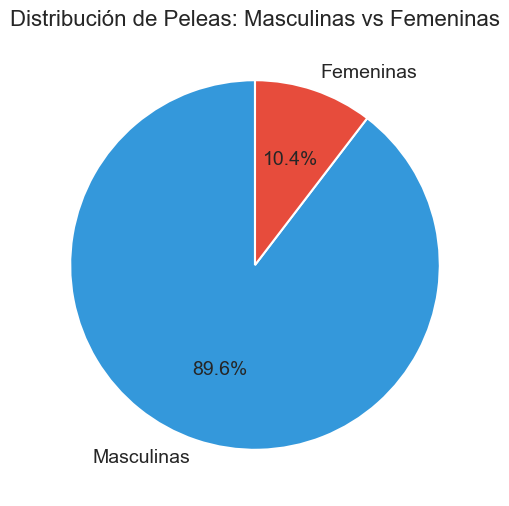
\includegraphics[width=0.6\textwidth]{DistribucionDePeleas.png}
    \caption{Distribución de peleas: Masculinas vs Femeninas.}
    \label{fig:peleas_dist}
\end{figure}

Dada esta marcada diferencia de volumen, se ha decidido centrar el análisis y el correspondiente modelo predictivo exclusivamente en las peleas masculinas, a fin de evitar sesgos y mantener el posterior análisis sobre un conjunto de datos homogéneo. Posteriormente, sobre este nuevo subconjunto, se evaluó la cantidad de datos faltantes.

Si bien el proceso de depuración definitivo se realizará tras un análisis exploratorio exhaustivo, se ha planteado un criterio preliminar para el manejo de valores faltantes y la selección de características, orientado específicamente a responder las tres preguntas centrales del trabajo. 

\begin{figure}[H]
    \centering
    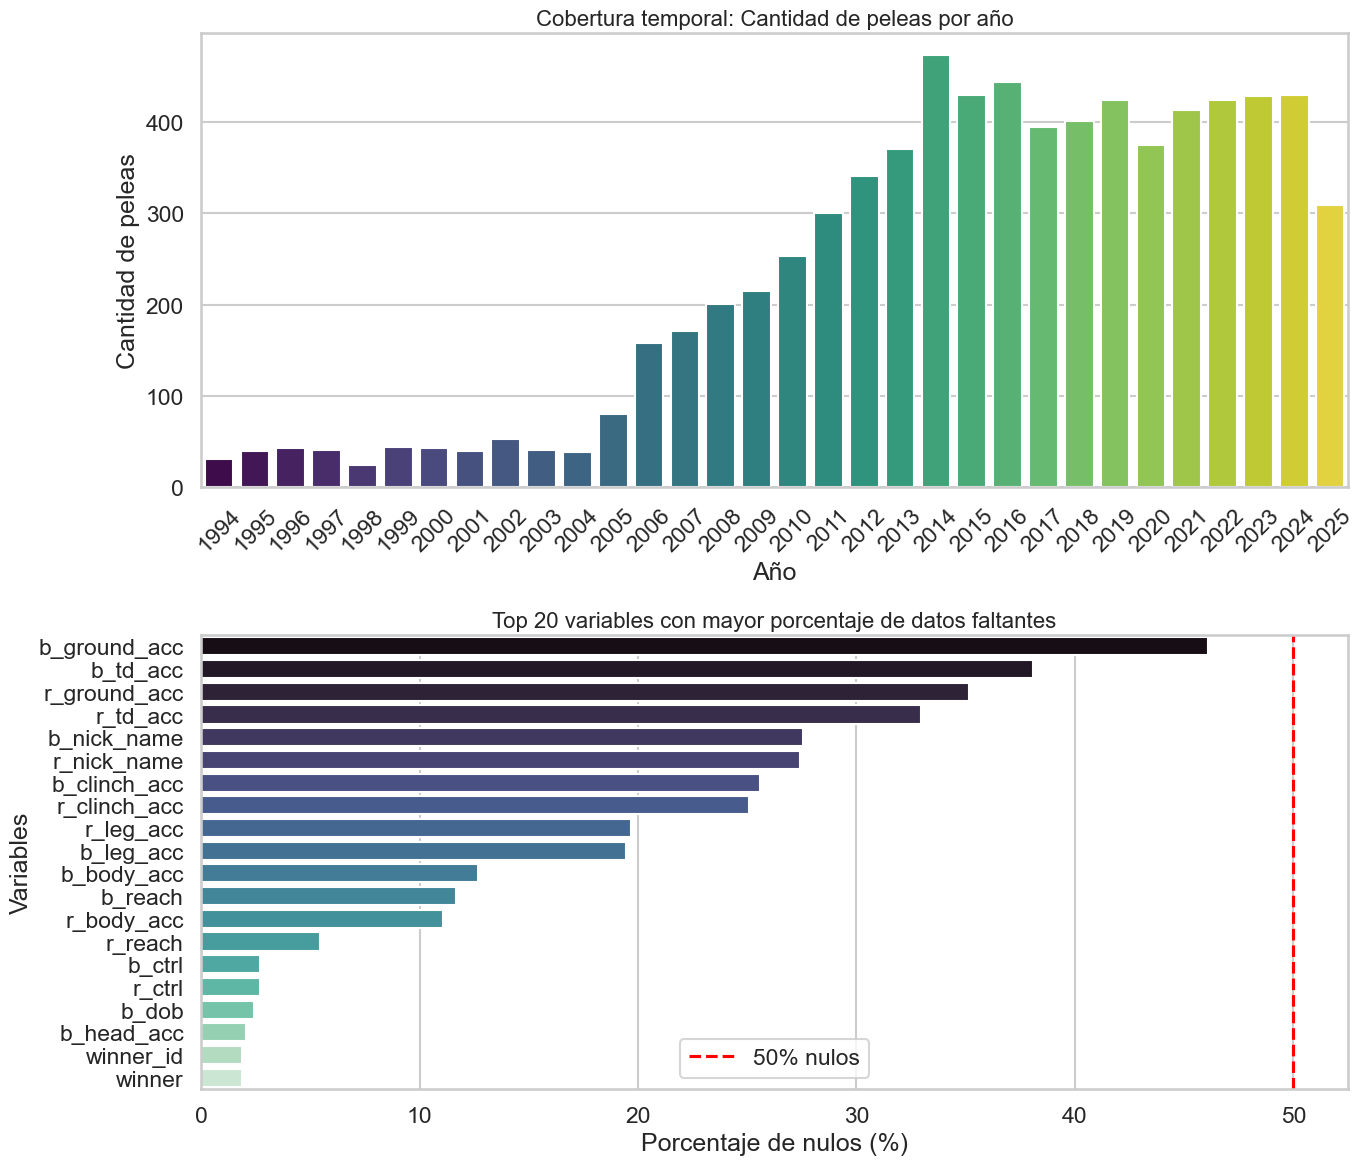
\includegraphics[width=1\textwidth]{DistribucionDeNulos.png}
    \caption{Cobertura temporal de las peleas por año (arriba) y análisis de atributos con mayor porcentaje de datos faltantes (abajo).}
    \label{fig:cobertura_y_nulos}
\end{figure}

Previamente al modelado, también resulta valioso entender la dinámica estructural de los enfrentamientos. Como se observa en la Figura \ref{fig:estructura_combate}, se exploraron cuatro métricas contextuales clave: la cantidad de peleas por división de peso, las vías o métodos de cierre del combate, la distribución del round de finalización y la duración total en minutos. Este análisis general permite vislumbrar cómo tienden a resolverse los encuentros en los distintos rangos de peso y tiempo, estableciendo una base descriptiva sólida.

\begin{figure}[H]
    \centering
    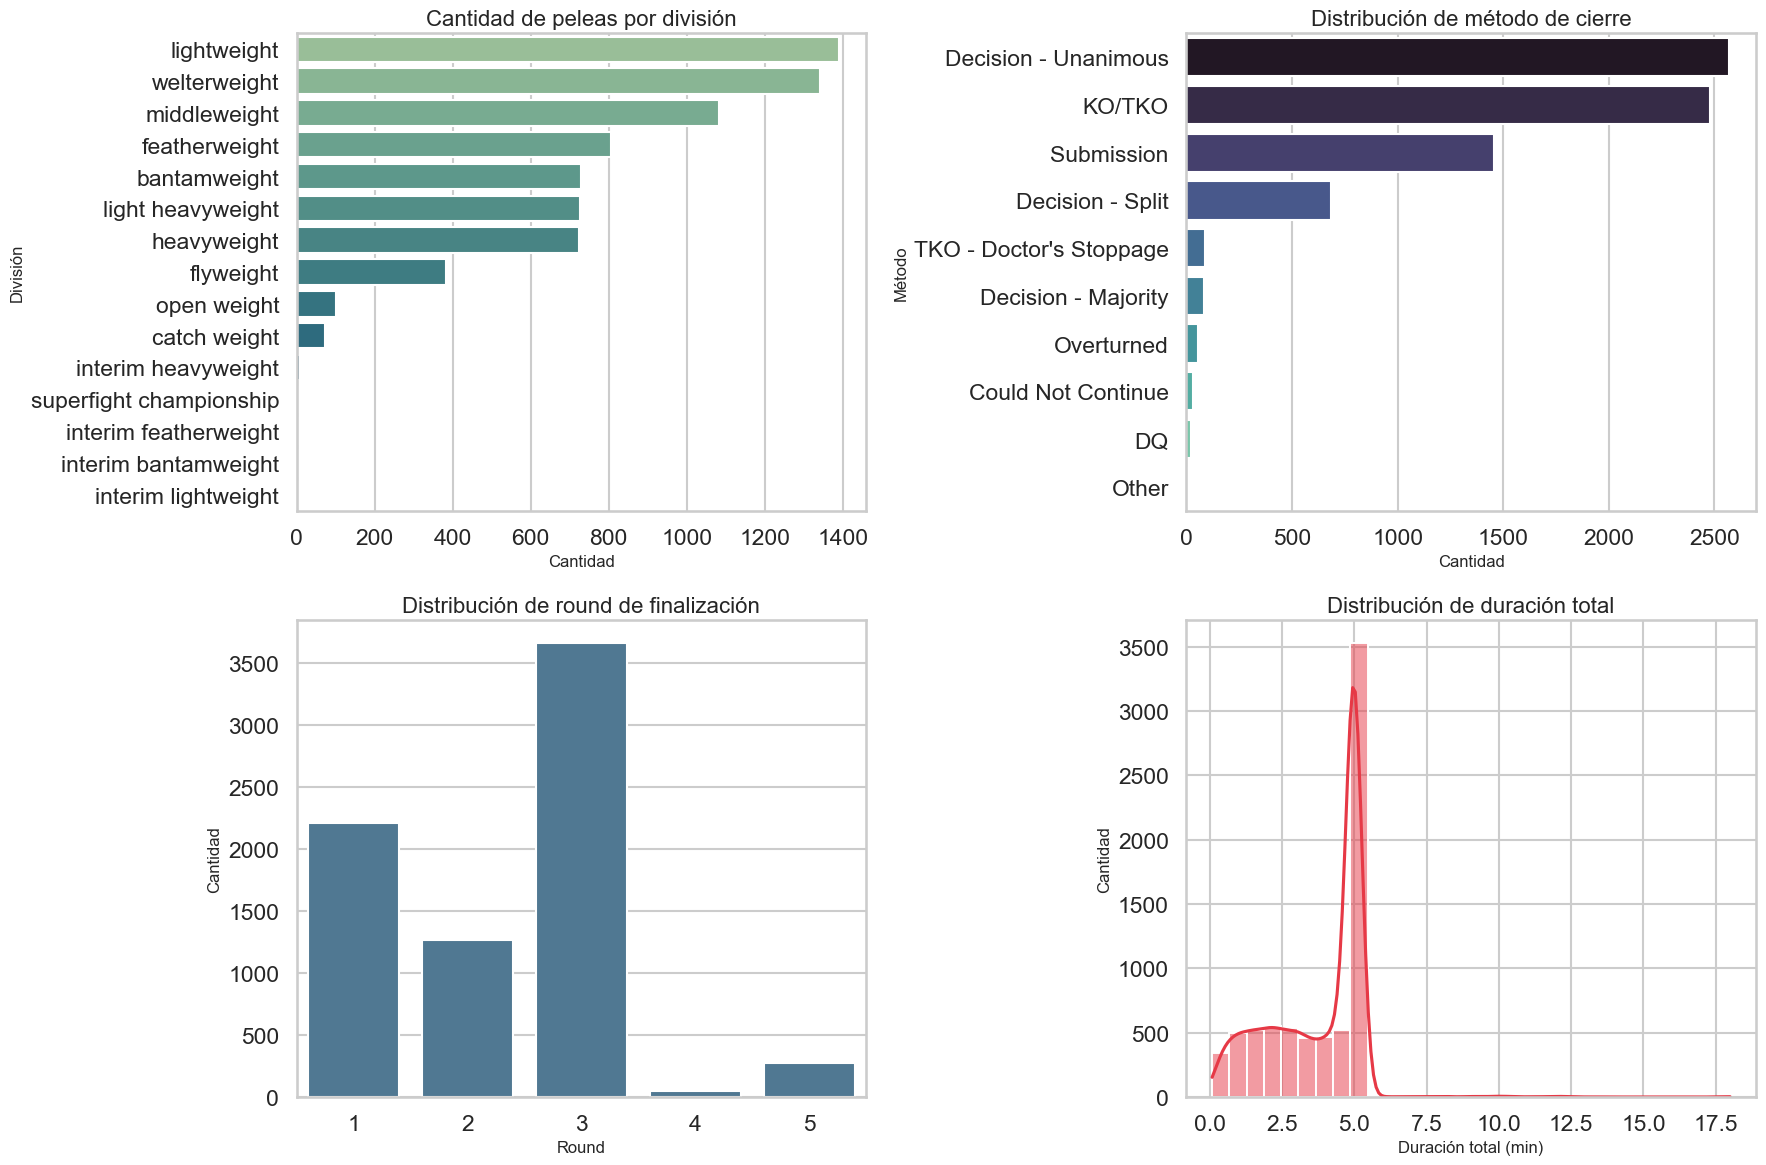
\includegraphics[width=1\textwidth]{Imagen3.png}
    \caption{Análisis exploratorio: cantidad de peleas por división, método de cierre, round de finalización y duración de los combates.}
    \label{fig:estructura_combate}
\end{figure}

A continuación, se detalla el enfoque proyectado para cada una de las preguntas de investigación:

\subsection*{1. ¿Qué luchador tiene mayor probabilidad de ganar una pelea dada?}
Dado que este problema se abordará como una tarea de clasificación binaria, es de vital importancia utilizar únicamente información disponible \textbf{antes} de que ocurra el combate. 

Por lo tanto, se descartarán todas las estadísticas recolectadas \textit{durante} la pelea en sí (tales como la cantidad de golpes conectados en un round específico, tiempos de control y porcentajes de precisión). Las variables a conservar incluyen metadatos del evento (división, si es por el título, cantidad de rounds) y características pre-combate de cada peleador (récord de victorias/derrotas, postura, edad calculada a partir de la fecha de nacimiento y atributos físicos). 

Los valores faltantes en estas variables retenidas se imputarán empleando sus respectivas modas o medianas segmentadas por división. Finalmente, se filtrarán estrictamente las peleas sin un ganador definido para poder entrenar adecuadamente el modelo clasificador (ej. Regresión Logística o Random Forest).

\subsection*{2. Si soy un luchador con determinadas características, ¿qué tipo de pelea me conviene aceptar?}
En este escenario, el objetivo es recomendar el contexto de pelea que maximice la probabilidad de victoria. 
Se mantendrán las características físicas y de historial del luchador (previamente imputadas), centrando el análisis en las variables de contexto: cantidad de rounds pactados, división, si hay un título en juego y el referí. 

Para variables de contexto con datos faltantes (por ejemplo, la cantidad de rounds), se realizará una imputación basada en la naturaleza del combate (utilizando la variable \textit{title\_fight} como pista, ya que estas suelen ser a 5 rounds). En el caso de valores ausentes en el campo del árbitro, se generará una categoría independiente (\textit{Unknown}). Se construirá un modelo que prediga la probabilidad de ganar en función de las características fijas del luchador interactuando con las distintas combinaciones posibles del contexto de pelea.

\subsection*{3. Si soy una persona con determinadas características, ¿qué estilo me conviene practicar?}
Esta pregunta requiere cambiar el nivel de análisis: de un enfoque por combate individual a un perfil agregado por luchador. 
Para determinar un estilo de pelea (por ejemplo, \textit{Striker} puro, \textit{Grappler} o \textit{Balanceado}), se utilizarán estadísticas históricas acumuladas de cada combatiente (promedio de golpes significativos, derribos y sumisiones). 

Al crear este nuevo dataset agrupado por luchador, aquellos registros mínimos que presenten valores nulos en columnas esenciales de golpes (como \textit{sig\_str\_landed}) podrán ser directamente eliminados sin impacto significativo (representan menos del 1\% del conjunto). Una vez consolidada la base limpia, se aplicarán algoritmos de agrupamiento (ej. \textit{K-Means}) sobre las estadísticas ofensivas para asignar un estilo definitivo a cada peleador. La recomendación final consistirá en buscar en este espacio a los luchadores físicamente más similares a la persona consultante que posean un porcentaje de victorias superior al 50\%, recomendando el estilo predominante de este subgrupo exitoso.

\section{Información complementaria del dataset}

En complemento a la información principal consolidada, los archivos secundarios adjuntos en la descarga original listan por separado a los luchadores, peleas y eventos, lo que abre posibilidades para cruzar datos en bases más segmentadas si el trabajo lo requiriese a futuro. 

La gran riqueza técnica del conjunto de datos radica en su profunda distinción estadística para cada rincón del octágono, permitiendo medir y comparar en igualdad de condiciones el impacto en cabeza, cuerpo, manejo en diferentes distancias y tiempos de control de cada competidor.

\end{document}